
\chapter{Testing intelligent systems}\label{ch:difftest}

\setlength{\epigraphwidth}{0.80\textwidth}
\epigraph{``If we use, to achieve our purposes, a mechanical agency with whose operation we cannot efficiently interfere\ldots then we had better be quite sure the purpose put into the machine is the purpose which we really desire.''}{\begin{flushright}--Norbert \citet{wiener1960some}, \href{https://www.ias.ac.in/article/fulltext/reso/004/01/0080-0088}{\textit{Some moral and technical consequences of automation}}~\end{flushright}}

Today's deep neural networks are capable of learning a broad range of functions, but have specific weaknesses. Training neural networks which can robustly transfer to new domains where the training and test distributions are highly dissimilar poses a significant challenge. These models are often susceptible to failure when presented with carefully crafted inputs. However, the same gradient-based optimization techniques used for training neural networks can also be exploited to probe their failure modes.

In software engineering, techniques for software testing are becoming increasingly automated and general-purpose. Tests help prevent regressive behavior and are a form of specification in which the developer communicates the intended result of running a program. While essential for validating a program's correctness, tests are often cumbersome to implement. Techniques in coverage-guided fuzzing have enabled developers to write fewer tests with higher coverage. This is made possible by automated testing.

In this chapter, we will explore the relationship between testing in machine learning and software engineering. We will see how the notion of adversarial testing shares a curious resemblance to fuzz testing in software engineering. In particular, we show how probabilistic sampling and constrained optimization can be seen as an extension of property-based testing (PBT) for adversarial training of differentiable programs, and propose a PBT algorithm which incorporates features of probabilistic programming and gradient-based optimization.

\section{Unit Testing}

\noindent In traditional unit testing, most tests are written in the following manner:
%
\begin{kotlinlisting}
fun unitTest(subroutine: (Input) -> Output) {
    val input = Input() // Construct an input
    val expectedOutput = Output() // Construct an output
    val actualOutput = subroutine(input)
    assert(expectedOutput == actualOutput) { "Expected $expectedOutput, got $actualOutput"}
}
\end{kotlinlisting}
%
When carefully applied, unit testing can be an effective method for detecting bugs and validating the author's belief about preconditions and postconditions. The trouble is, someone needs to write a bunch of test cases for it to work. In addition, it only tests subprograms, and must be updated whenever the program changes. This has the unintended side effect of decreasing agility, discouraging refactoring, or discarding prior work when tests become obsolete.

\section{Integration Testing}

\noindent In integration testing, we are more concerned about the overall behavior of a program, rather than the specific behavior of its subroutines. Consider the following example:

\begin{kotlinlisting}
fun <I, O> integrationTest(program: (I) -> O, inputs: Set<I>, checkOutput: (O) -> Boolean) =
    inputs.forEach { input: I ->
        try {
            val output: O = program(input)
            assert(checkOutput(output)) { "Postcondition failed on $input, $output" }
        } catch (exception: Exception) {
            assert(false) { exception }
        }
    }
\end{kotlinlisting}
%
With this strategy, there are fewer tests to write down, since we only care about end-to-end behavior. Integration testing simply checks a program for terminating exceptions and simple post conditions. For this reason, it is often too coarse-grained.

For simplicity, in the following sections, we will only consider examples of programs which are pure functions, i.e. which have no external state and produce no side effects.

\section{Fuzz Testing}

Fuzz testing is an automated testing methodology which generates random inputs to test a given program. For example, consider the following test:
%
\begin{kotlinlisting}
fun <I, O> fuzzTest(program: (I) -> O, oracle: (I) -> O, rand: () -> I) =
    repeat(1000) {
        val input: I = rand()
        assert(program(input) == oracle(input)) { "Oracle and program disagree on $input" }
    }
\end{kotlinlisting}
%
The trouble is, we need an oracle, an often unreasonable assumption. This is known as the \textit{test oracle problem}. But even if we had an oracle, since the space of inputs is often large, it can take a long time to find an output where they disagree. Since a single call to \inline{program(i)} can be quite expensive in practice, this method can also be quite inefficient.

\section{Property-based Testing}\label{subsec:property-based-testing}

Property-based testing~\citep{fink1997property} (PBT) attempts to mitigate the test oracle problem by using \textit{properties}. It consists of two phases, searching and shrinking. Users specify a property over all outputs and the test fails if a counterexample can be found:
%
\begin{kotlinlisting}
fun <I, O> gen(program: (I) -> O, property: (O) -> Boolean, rand: () -> I) =
    repeat(1000) {
        val randomInput: I = rand()

        assert(property(program(randomInput))) {
            val shrunken = shrink(randomInput, program, property)
            "Minimal input counterexample of property: $shrunken"
        }
    }
\end{kotlinlisting}
%
Roughly speaking, \inline{shrink} attempts to minimize the counterexample.
%
\begin{kotlinlisting}
tailrec fun <I, O> shrink(failure: I, program: (I) -> O, property: (O) -> Boolean): I =
    if (property(program(decrease(failure)))) failure // Property holds once again
    else shrink(decrease(failure), program, property) // Decrease until property holds
\end{kotlinlisting}
%
For example, given a \inline{program: (Float) -> Any}, we might implement \inline{decrease} like so:
%
\begin{kotlinlisting}
fun decrease(failure: Float): Float = failure - failure / 2
\end{kotlinlisting}
%
\begin{figure}
\begin{tikzpicture}
\begin{axis}[title={Log errors between AD and SD on $f(x) = \frac{\sin(\sin(\sin(x))))}{x} + x\sin(x) + \cos(x) + x$}, width=0.95\textwidth, height=10cm, xlabel=$x$, ylabel=$\log_{10}(\Delta)$, legend pos=south east, align=center]
\addplot table [mark=none, x index=0, y index=1, col sep=comma] {../data/adsd_comparison.csv};
\addlegendentry{$\Delta$(SD, AP) $\approx\Delta$(AD, IP)}
\addplot table [mark=none, x index=0, y index=2, col sep=comma] {../data/adsd_comparison.csv};
\addlegendentry{$\Delta$(AD, SD)}
\addplot table [mark=none, x index=0, y index=3, col sep=comma] {../data/adsd_comparison.csv};
\addlegendentry{$\Delta$(FD, AP)}
\end{axis}
\end{tikzpicture}
\caption{We compare numerical drift between AD and SD over a swollen expression using fixed precision and arbitrary precision (AP). AD and SD both exhibit relative errors (i.e. with respect to each other) several orders of magnitude lower than their absolute error. These results are consistent with the findings of ~\citet{laue2019equivalence}.\vspace{-10pt}}
\label{fig:pbt_comparison}
\end{figure}
%
Consider \autoref{fig:pbt_comparison}, which portrays the log difference between various forms of computational differentiation (evaluated using standard 32-bit precision) and AP (computed to 30 significant figures).\hspace{-.08em}\footnote{To calculate AP, we symbolically derive the function and numerically evaluate it using \hyperref[sec:fdm]{finite difference approximation} and MacLaurin series expansion of sine and cosine.} Given two algorithms for calculating the derivative, a property-based test might check whether the absolute difference is bounded over all inputs.

The trouble is, finding the right properties to test can be highly sensitive, and requires a lot of effort and domain-specific expertise. In addition, the user must specify a custom shrinker, which is unclear how to implement efficiently. What if there were a better way?

\section{Metamorphic testing}\label{subsec:metamorphic-testing}

It is often the case we would like to test the behavior of a program without providing an exhaustive specification. Many naturally-occurring generative processes exhibit a kind of local invariance -- small changes to the input do not drastically change the output. We can exploit this property to design general-purpose fuzzing methods given a small set of inputs and outputs. Metamorphic testing (MT) is a property testing methodology which addresses the test oracle problem and the challenge of cheaply discovering bugs in the low-data regime. It has been successfully applied in testing driverless cars~\citep{zhou2019metamorphic, pei2017deepxplore, tian2018deeptest} and other stateful deep learning systems~\citep{du2018deepcruiser}.

First, let us consider the following concrete example, from \citet{tian2018deeptest}: suppose we have implemented a program which takes an image from a vehicle while driving, and predicts the simultaneous steering angle of the vehicle. Given a single image and the corresponding ground-truth steering angle from an oracle (e.g. a human driver or simulator), our program should preserve invariance under various image transformations, such as limited illumination changes, linear transformations or additive noise below a certain threshold. Intuitively, the steering angle should remain approximately constant, regardless of any single transformation or sequence of transformations applied to the original image which satisfy our chosen criteria. If not, this is a strong indication our program is not sufficiently robust and may not respond well to the sort of variability it may encounter in an operational setting.

Metamorphic testing can be expressed as follows: Given an oracle $\mathbf P: \mathcal I \rightarrow \mathcal O$, and a set of inputs $\mathbf X = \{\mathbf{x}^{(1)}, \dots, \mathbf{x}^{(z)}\}$ and outputs $\mathbf Y = \{\mathbf{y}^{(1)} = \mathbf{P}(\mathbf{x}^{(1)}), \dots, \mathbf{y}^{(z)} = \mathbf{P}(\mathbf{x}^{(z)})\}$, a metamorphic relation (MR) is a relation $\mathcal R \subset \mathcal I^z \times \mathcal O^z$ where $z \geq 2$. In the simplest case, an MR is an equivalence relation $\mathcal R$, i.e.: $\langle \mathbf x, \mathbf y, \mathbf x', \mathbf y' \rangle \in \mathcal R \Leftrightarrow \mathbf x \sim_{\mathcal R} \mathbf x' \Leftrightarrow \mathbf P(\mathbf x) \approx \mathbf P(\mathbf x')$.

Suppose our MR is $\forall \varphi \in \mathcal I: ||\mathbf\varphi|| \leq \varepsilon, \mathbf P(\mathbf x) \approx \mathbf P(\mathbf x' = \mathbf x + \varphi) \approx \mathbf y$. Given a program $\mathbf{\hat P}$ and a comparatively small set of inputs $\mathbf X$ and outputs $\mathbf Y$ from our oracle $\mathbf P$, the MR produces a set $\mathbf X', |\mathbf X| \ll |\mathbf X'|$ on which to test $\mathbf{\hat P}$, without requiring corresponding outputs from $\mathbf P$. If we can show $\exists \mathbf x' \in \mathbf X' \mid \mathbf{\hat P}(\mathbf x') \not\approx \mathbf P(\mathbf x)$, this implies at least one of the following:

\begin{enumerate}
\item $\langle \mathbf x, \mathbf P(\mathbf x), \mathbf x', \mathbf P(\mathbf x')\rangle \notin \mathcal R$, i.e. our assumptions were invalid
\item $\mathbf{\hat P}(\mathbf x') \not\approx \mathbf{P}(\mathbf x')$, i.e. the program under test is unsound
\end{enumerate}
%
In either case, we have obtained useful information. If our assumptions were invalid, we can strengthen the invariant, $\mathcal R$, by removing the counterexample. Otherwise, we have detected an error and can adjust the program to ensure compliance -- both are useful outcomes.

Consider the following example of an MT which uses an equivalence-based MR:

\begin{kotlinlisting}
fun <I, O> mrTest(program: (I) -> O, mr: (I, O, I, O) -> Boolean, rand: () -> Pair<I, O>) =
    repeat(1000) {
        val (input: I, output: O) = rand()
        val tx: (I) -> I = genTX(program, mr, input, output)
        val txInput: I = tx(input)
        val txOutput: O = program(txInput)
        assert(mr(input, output, txInput, txOutput)) {
            "<$input, $output> not related to <$txInput, $txOutput> by $mr ($tx)"
        }
    }
\end{kotlinlisting}
%
The trouble is, generating valid transformations is a non-trivial exercise. We could try to generate random transformations until we find one which meets our criteria:
%
\begin{kotlinlisting}
fun <I, O> genTX(program: (I) -> O, mr: (I, O, I, O) -> Boolean, i: I, o: O): (I) -> I {
    while (true) {
        val tx: (I) -> I = sampleRandomTX()
        val txInput: I = tx(i)
        val txOutput: O = program(txInput)
        if (mr(i, o, txInput, txOutput)) return tx
    }
}
\end{kotlinlisting}

But this would be very inefficient and depending on the type of input and output, is not guaranteed to terminate. We could handcraft a transformation, but this requires extensive domain knowledge. Instead, we should seek a more principled, computationally efficient and general purpose method of mutating an input in our dataset to discover invalid outputs.

\section{Adversarial Testing}

This leads us to adversarial testing. In the general case, we are given an input-output pair from an oracle and a program approximating the oracle, but not necessarily the oracle itself. Our goal is to find a small change to the input of a function, which produces the largest change to its output, relative to the original output.

Imagine a function $\mathbf{\hat P}: \mathbb R^m \rightarrow \mathbb R$, each component $g_1, ..., g_{m}$ of which we seek to change by a fixed amount so as to produce the largest output value $\mathbf{\hat P}(g'_1, ..., g'_{m})$ directly. Suppose for each input parameter $g_1, \ldots, g_{m}$, we have one of three choices to make: either we can increase the value by $c$, decrease the value by $c$, or leave it unchanged. We are given no further information about $\mathbf{\hat P}$. Consider the na\"ive solution, which tries every combination of variable perturbations and selects the input corresponding to the greatest output value:

\begin{algorithm}[H]
\caption{Brute Force Adversary}
\label{alg:bf_adversary}
\begin{algorithmic}[1]
\Procedure{BfAdversary}{$\mathbf{\hat P}: \mathbb{R}^m \rightarrow \mathbb{R}$, $c: \mathbb R$, $g_1: \mathbb R$, $g_2: \mathbb R$, $\ldots$, $g_{m}: \mathbb R$}: $\mathbb{R}^m$
\If {$m = 1$} \Comment{Evaluate $\mathbf{\hat P}$ and return the best variable perturbation}
\State \Return $\operatorname{argmax}\{\mathbf{\hat P}(g_1 + c), \mathbf{\hat P}(g_1 - c), \mathbf{\hat P}(g_1)\}$
\Else \Comment{Partially apply candidate perturbation and recurse}
\State \Return $\operatorname{argmax}\{\mathbf{\hat P}(g_1 + c) \circ$\Call{BfAdversary}{$\mathbf{\hat P}(g_1 + c), c, g_2, \ldots, g_{m}$},\newline
\hspace*{10em} $\mathbf{\hat P}(g_1 - c)\circ$\Call{BfAdversary}{$\mathbf{\hat P}(g_1 - c), c, g_2, \ldots, g_{m}$},\newline
\hspace*{10em} $\mathbf{\hat P}(g_1)\circ$\Call{BfAdversary}{$\mathbf{\hat P}(g_1), c, g_2, \ldots, g_{m}$}$\}$
\EndIf
\EndProcedure
\end{algorithmic}
\end{algorithm}

As we can see, algorithm \autoref{alg:bf_adversary} is $\mathcal{O}(3^m)$ with respect to $\mathbf{\hat P}$ -- not a very efficient search routine, especially if we want to consider a larger set of perturbances. Clearly, if we want to find the best direction to update $\mathbf g$, we need to be more careful about how we perform the search.

Even if we cannot compute a closed-form derivative for $\mathbf{\hat P}$, if $\mathbf{\hat P}$ is differentiable almost everywhere, we can still use numerical differentiation to approximate pointwise values of its derivative. Consider algorithm \autoref{alg:fd_fuzz}, a refinement of algorithm \autoref{alg:bf_adversary} which uses the \hyperref[sec:fdm]{finite difference method} to approximate the derivative with respect to each component of the input. This tells us how to minimally change the input to produce the largest output in reach, without needing to exhaustively check every perturbation.

\begin{algorithm}[H]
\caption{Finite Difference Adversary}
\label{alg:fd_fuzz}
\begin{algorithmic}[1]
\Procedure{FdAdversary}{$\mathbf{\hat P}: \mathbb{R}^m \rightarrow \mathbb{R}$, $c: \mathbb R$, $g_1: \mathbb R$, $g_2: \mathbb R$, $\ldots$, $g_{m}: \mathbb R$}: $\mathbb{R}^m$
\If {$m = 1$} \Comment{Compute finite (centered) difference and perform gradient ascent}
\State \Return $g_1 + \frac{\mathbf{\hat P}(g_1 - c) - \mathbf{\hat P}(g_1 + c)}{2c}$
\Else \Comment{Apply single-step gradient ascent using componentwise finite difference}
\State \Return $g_1 + \frac{\mathbf{\hat P}(g_1 - c, 0, \ldots) - \mathbf{\hat P}(g_1 + c, 0, \ldots)}{2c}$, \Call{FdAdversary}{$\mathbf{\hat P}, c, g_1, \ldots, g_{m}$}
\EndIf
\EndProcedure
\end{algorithmic}
\end{algorithm}

We now have a procedure that is $\mathcal{O}(m)$ with respect to $\mathbf{\hat P}$, but must be recomputed for each input -- we can still do better by assuming further structure on $\mathbf{\hat P}$. Furthermore, we have not yet incorporated any form of constraint on the input values. Perhaps we can combine the notion of metamorphic testing seen in \autoref{subsec:metamorphic-testing} with constrained optimization to accelerate the search for adversarial examples.

During backpropagation we perform gradient descent on a differentiable function with respect to its parameters for a specific set of inputs. In gradient-based adversarial testing, we perform gradient ascent on a loss function with respect to the inputs using a fixed parameter setting. Suppose we have a differentiable vector function $\mathbf{\hat P}: \mathbb{R}^m\rightarrow\mathbb{R}^n$, defined as follows:
%
\begin{equation} \tag{\autoref{eq:recursive_parametric_eq} revisited}
\mathbf{\hat P}_k(\mathbf{x}; \bm\Theta) = \begin{cases} \mathbf{\hat p}_1(\Theta_1)\circ\mathbf{x} &\text{if } k=1\\ \mathbf{\hat p}_k(\Theta_k)\circ \mathbf{\hat P}_{k}(\bm\Theta_{[1, k]})\circ\mathbf{x}&\text{if } k > 1 \end{cases} \\
\end{equation}
%
In deep learning, given pairs $\mathbf{X} = \{\mathbf{x}^{(1)}, \dots, \mathbf{x}^{(z)}\}, \mathbf{Y} = \{\mathbf{y}^{(1)} = \mathbf{P}(\mathbf{x}^{(1)}), \dots, \mathbf{y}^{(z)} = \mathbf{P}(\mathbf{x}^{(z)})\}$ we want to find $\bm\Theta^* = \argmin{\boldsymbol{\Theta}}\mathcal{L}\big(\mathbf{\hat P}_k(\mathbf{x}^{(i)}; \bm\Theta), \mathbf{y}^{(i)}\big)$ which is typically achieved by performing stochastic gradient descent on the loss with respect to the model parameters:
%
\begin{equation} \tag{\autoref{eq:stochastic_grad_descent} revisited}
\bm\Theta \leftarrow \bm\Theta - \alpha\frac{1}{z}\nabla_{\bm\Theta} \sum_{i=1}^z\mathcal{L}\big(\mathbf{\hat P}_k(\mathbf{x}^{(i)}; \bm\Theta), \mathbf{y}^{(i)}\big)
\end{equation}
%
We can solve for the gradient with respect to $\bm\Theta$ by multiplying the Jacobians (\autoref{eq:vfun_chain_rule}), $\mathcal{J}_{\mathbf{p}_1} \cdots \mathcal{J}_{\mathbf{p}_k}$. In white box adversarial learning, we are given a fixed $\bm\Theta$~\footnote{In contrast with backpropagation, where the parameters $\bm\Theta$ are updated.} and control the value of $\mathbf x$, so we can rewrite $\mathbf{\hat P}_k(\mathbf{x}^{(i)};\bm\Theta)$ instead as $\mathbf{\hat P}(\mathbf x)$, and take the gradient directly with respect to $\mathbf x$. Our objective is to find the ``worst'' $\mathbf x$ within a small distance of any $\mathbf x^{(i)}$, i.e. where $\mathbf{P}(\mathbf x)$ least resembles $\mathbf{\hat P}(\mathbf x)$. More concretely, this can be expressed as,
%
\begin{equation}
\mathbf{x}^* = \argmax{\mathbf{x}}\mathcal{L}\big(\mathbf{\hat P}(\mathbf{x}), \mathbf{y}^{(i)}\big) \text{ subject to } CS = \{\mathbf{x} \in \mathbb{R}^m \text{ s.t. } ||\mathbf{x}^{(i)} - \mathbf{x}||_p    < \epsilon\}
\end{equation}
%
To do so, we can initialize $\mathbf{x} \sim U[CS]$ and perform projected gradient ascent on the loss:
%
\begin{equation}\label{eq:projected_gd}
\mathbf x \leftarrow \bm\Phi_{CS}\Big(\mathbf x + \alpha\mathbf\nabla_{\mathbf x} \mathcal{L}\big(\mathbf{\hat P}(\mathbf{x}), \mathbf{y}^{(i)}\big)\Big) \text{, where }
\bm\Phi_{CS}(\mathbf \phi') = \argmin{\mathbf \phi \in CS}\frac{1}{2}||\mathbf \phi - \mathbf \phi'||^2_2
\end{equation}
%
Henceforth we shall refer to $\mathcal{L}\big(\mathbf{\hat P}(\mathbf{x}), \mathbf{y}^{(i)}\big)$ as $\mathcal{L}(\mathbf x)$. Imagine a single test $\mathbf{T}: \mathbb{R}^m \times \mathbb{R} \rightarrow \mathbb{B}$:
%
\begin{equation} \label{eq:output_constraint_example}
\mathbf T(\mathbf{x}, C) = \mathcal{L}(\mathbf{x}) < C
\end{equation}
%
Where $C \in \mathbb{R}$. How should we find a set of inputs that break our test given a fixed computational budget (i.e.\ constant number of program evaluations)? More concretely:
%
\begin{equation}
\{ D_\mathbf T: \mathbf x \in CS \mid \mathbf{\hat P}(\mathbf x) \implies \neg \mathbf T \}, maximize |D_\mathbf T|
\end{equation}
%
Assuming zero knowledge about the program's implementation or the data distribution, $D_{\mathbf{\hat P}}$, we can do no better than random search~\citep{wolpert1997no}. Given access to $\mathbf{\hat P}$'s implementation, we could use classical fuzzing techniques to prioritize the search for inputs more likely to violate $\mathbf T$. Assuming the program is differentiable, given input-output access but not the source code, we can still use zeroth order optimization techniques to approximate the gradient. Given access to its implementation, we can accelerate the search by using automatic differentiation. Furthermore, given information about the data distribution, we could re-parameterize the distribution to initialize the search in promising regions of the input space. By assuming the program has previously been tested on common inputs, we might sample from the inverse training distribution $x \sim \frac{1}{D_{\mathbf{\hat P}}}$ to select low probability inputs, possibly more likely to elicit an error.

% Finally, we could train a neural network to predict inputs that were likely to cause a program to fail a given specification. As input, the network would take the function and test cases, and as its output, produce values that were likely to violate $T$.

\section{Generative Adversarial Testing}

What constitutes a good adversary? For an adversary to be considered a strong adversary, a significant fraction of her candidate inputs must break the program specification. To generate plausible test cases, not only must she be able to exploit weaknesses of the program, but ideally possess a good understanding of $p_{data}$.

Suppose we have a program $D: \mathbb{R}^h\rightarrow\mathbb{B}$, i.e. a binary classifier. How should we test its implementation, without providing an exhaustive specification, or some prior distribution over the inputs? One solution, known as a generative adversarial network~\citep{goodfellow2014gan} (GAN), proposes a generative adversary $G: \mathbb{R}^v\rightarrow\mathbb{R}^h$. The vanilla GAN objective can be expressed as a min-max optimization problem:

\begin{equation}
\min_G \max_D V(D, G) = \mathbb{E}_{\mathbf x \sim p_{data}(\mathbf x)}\big[\log D(\mathbf x)\big] + \mathbb{E}_{\mathbf z \sim p_{\mathbf z}(\mathbf z)}\big[\log\big(1 - D(G(\mathbf z))\big)\big]
\end{equation}

This objective can be optimized by sampling minibatches $\mathbf x \sim p_{data}(\mathbf x)$ and $\mathbf z \sim p_{G}(\mathbf z)$, then updating the parameters of $G$ and $D$ using their respective stochastic gradients:

\begin{equation}
\theta_D \leftarrow \theta_D + \nabla_{\theta_D}\frac{1}{m}\sum_{i=1}^m\Big[\log D(\mathbf x^{(i)}) + \log\Big(1 - D\big(G(\mathbf z^{(i)})\big)\Big)\Big]
\end{equation}

\begin{equation}
\theta_G \leftarrow \theta_G - \nabla_{\theta_G}\frac{1}{m}\sum_{i=1}^m \log\Big(1 - D\big(G(\mathbf z^{(i)})\big)\Big)
\end{equation}
%
\citet{albuquerque2019hgan} propose an augmented version of this game using multiple Discriminators which each receive a fixed, random projection $P_k(\cdot)$ of the Generator's output, and solves the following multi-objective optimization problem:
%
\begin{equation}
\min \mathbf{\mathcal{L}}_G(\mathbf x) = \left[l_1(\mathbf z), l_2(\mathbf z), \ldots, l_K(\mathbf z)\right] \text{, where } l_k = -\mathbb E_{z \sim p_z} \log D_k(P_k(G(z_k)))
\end{equation}
%
This can be achieved by using a variant of hypervolume maximization:
%
\begin{equation}
\nabla_\Theta \mathcal{L}_G = \sum_{k=1}^K \frac{1}{\eta - l_k}\nabla_\Theta l_k
\end{equation}

Where $\eta$ is a common, fixed upper bound on every $l_k$. Further GAN variants such as WGAN~\citep{arjovsky2017wgan}, MHGAN~\citep{turner2019mhgan}, et al. have proposed augmentations to the vanilla GAN to improve stability and sample diversity. GANs have been successfully applied in various domains from speech~\citep{donahue2019wavegan} to graph synthesis~\citep{wang2018graphgan}. One practical extension to the latter could be applying the GAN framework to program synthesis and compiler optimization by choosing a suitable metric and following the approach proposed by e.g.~\citet{adams2019learning, mendis2019compiler}.
%
\section{Probabilistic Adversarial Testing}

% Furthermore, we hypothesize that if a sufficiently large fraction of the input space existed where $T$ were false, then as we sample from that space, the probability of detection would approach 1:
%
% \begin{equation}
%     (\forall i \in I^\dagger, p(i) \implies \neg T) \implies \lim_{|x|\to \infty}Prob(\hat{T}=False) = 1
% \end{equation}
%

Let us consider an extension of classical fuzzing methods to differentiable functions on continuous random variables. First, we select $\mathbf{x}_j: \mathbb{R}^m \sim \mathcal S_m$ (e.g.\ uniform random prior, or using a meta-learner $\mathbf M: (\mathbb{R}^m \rightarrow \mathbb{R}^n) \times (\mathbb{R}^m \times \mathbb R \rightarrow \mathbb B) \rightarrow \mathbb{R}^m$ as input). If $\mathbf{\hat P}(\mathbf{x}^i)$ violates $\mathbf T$, we can append $\mathbf x^i$ to $D_\mathbf T$ and repeat. Otherwise, we update $\mathbf x$ following $\nabla_{\mathbf x}\mathcal{L}(\mathbf{x})$ and repeat until test failure, gradient descent convergence, or a fixed number of steps $C$ are reached before resampling $\mathbf{x}$ from $\mathcal S_m$. $C$ ensures each gradient descent trajectory terminates before exhausting the allotted computational budget. This procedure is described in \autoref{alg:prob_adversary}.

We hypothesize that if $\mathbf{\hat P}$'s implementation were indeed flawed and a counterexample to \autoref{eq:output_constraint_example} existed, as sample size increased, a subset of gradient descent trajectories would fail to converge at all, a subset would converge to local minima, and the remaining trajectories would discover inputs violating the program specification.

\begin{algorithm}[ht]
\caption{Probabilistic Generator}
\label{alg:prob_adversary}
\begin{algorithmic}[1]
\Procedure{ProbAdversary}{$\mathcal L: \mathbb R^m \rightarrow \mathbb R$, $\mathcal S_m$, budget: $\mathbb Z^+$}
\State $D_\mathbf T \gets \{\}, j \gets 0$
\While{$j \le$ budget}\Comment{Iterate until count exceeds our budget}
\State $\mathbf{x}_j \sim \mathcal S_m$\Comment{Sample from S}
\If {$\mathbf T\big(\mathbf{x}_j, \mathcal L(\mathbf{x}_j)\big)$} \Comment{Inside feasible set, perform gradient ascent}
\State $D_\mathbf T \gets D_\mathbf T$ $\cup$ \Call{DiffShrink}{$-\mathcal L, \mathbf{x}_j, \mathbf T$}
\Else \Comment{Outside feasible set, perform gradient descent}
\State $D_\mathbf T \gets D_\mathbf T$ $\cup$  \Call{DiffShrink}{$\mathcal L, \mathbf{x}_j, \mathbf T$}
\EndIf
\State $j \gets j + 1$
\EndWhile
\State \Return $D_\mathbf T$
\EndProcedure
\end{algorithmic}
\end{algorithm}

\begin{algorithm}[ht]
\caption{Differential Shrinker}
\label{alg:diff_adversary}
\begin{algorithmic}[1]
\Procedure{DiffShrink}{$\mathcal L: \mathbb R^m \rightarrow \mathbb R$, $\mathbf{x}_1: \mathbb R^m$}
\State $i \gets 1$
\State $t_1 \gets \mathbf T\big(\mathbf x_1, \mathcal L(\mathbf x_1)\big)$ \Comment{Store initial state to detect when test flips.}
\While {$i \leq I_{max}$ \textbf{and} $\mathbf ||\mathbf x_i - \mathbf x_{i-1}||_2^2 < \epsilon$} \Comment{While in budget and not converged.}
\State $\mathbf x_i \gets \bm\Phi_{CS}\big(\mathbf x_{i-1} - \alpha\mathbf\nabla_{\mathbf x_{i-1}} \mathcal{L}(\mathbf{x}_{i-1})\big)$ \Comment{PGD step (\autoref{eq:projected_gd})}
\If {$\mathbf T\big(\mathbf{x}_i, \mathcal L(\mathbf{x}_i)\big) \neq t_1$} \Comment{Boundary value was found.}
\State \Return $\{\mathbf{x}_{i-1}\}$ \Comment{Return previous iterate.}
\EndIf
\State $i \gets i + 1$
\EndWhile
\State \Return \textbf{if } $\neg t_1$ \textbf{ then } $\{\mathbf x_{i-1}\}$ \textbf{ else } $\varnothing$ \Comment{Return last iterate or $\varnothing$ if test passed.}
\EndProcedure
\end{algorithmic}
\end{algorithm}

To evaluate our algorithm, we train a polynomial regressor \autoref{sec:poly_reg} on input-output pairs from a set of random algebraic expressions. These expressions are produced by generating perfect binary trees of depth 5, whose leaf nodes contain with equal probability either (1) an alphabetic variable or (2) a random 64-bit IEEE 754 floating point number uniformly sampled in the range $[-1, 1]$. The internal nodes contain with equal probability a random operator in the set $\{+, \times\}$. Our expression generator with type $G_e: \mathbb{N}^+\times\mathbb{Z} \rightarrow \mathbb{R}^{[1, 26]} \rightarrow \mathbb{R}$ takes a depth $\delta$, a random seed $\psi$, and returns a scalar-valued function.

\begin{equation}\label{eq:btree_gen}
G_e(\delta, \psi) = \begin{cases}
\delta\sim\{a,b,..z\} & \text{if } \delta \leq 0 \text{ and } \gamma\sim_\psi\{\text{True, False}\},\\
\chi\sim U(-1, 1) & \text{if } \delta \leq 0 \text{ and } \gamma\sim_\psi\{\text{True, False}\},\\
G(\delta-1, \psi) + G(\delta-1, \psi) & \text{if } \delta > 0 \text{ and } \gamma\sim_\psi\{\text{True, False}\},\\
G(\delta-1, \psi) \times G(\delta-1, \psi) & \text{if } \delta > 0 \text{ and } \gamma\sim_\psi\{\text{True, False}\}.\\
\end{cases}
\end{equation}

Our training set consists of input-output pairs produced by binding the set of free variables belonging to the same datatype and numerical range as the constants, evaluating the expression on input values in the range $[-1, 1]$ and rescaling all output values to in the range $[-1, 1]$ using min-max normalization, i.e. $\tilde{G}_e(\delta, \psi)= \frac{G_e(\delta, \psi)}{\max |G_e(\delta, \psi)[-1, 1]|}$. For each expression in our dataset, we then train a polynomial regressor to convergence using SGD. Then, for both adversarial testing and uniform random sampling strategies, compare the average number of violations detected per evaluation as a function of input dimension and error tolerance.

\begin{figure}[H]
\centering
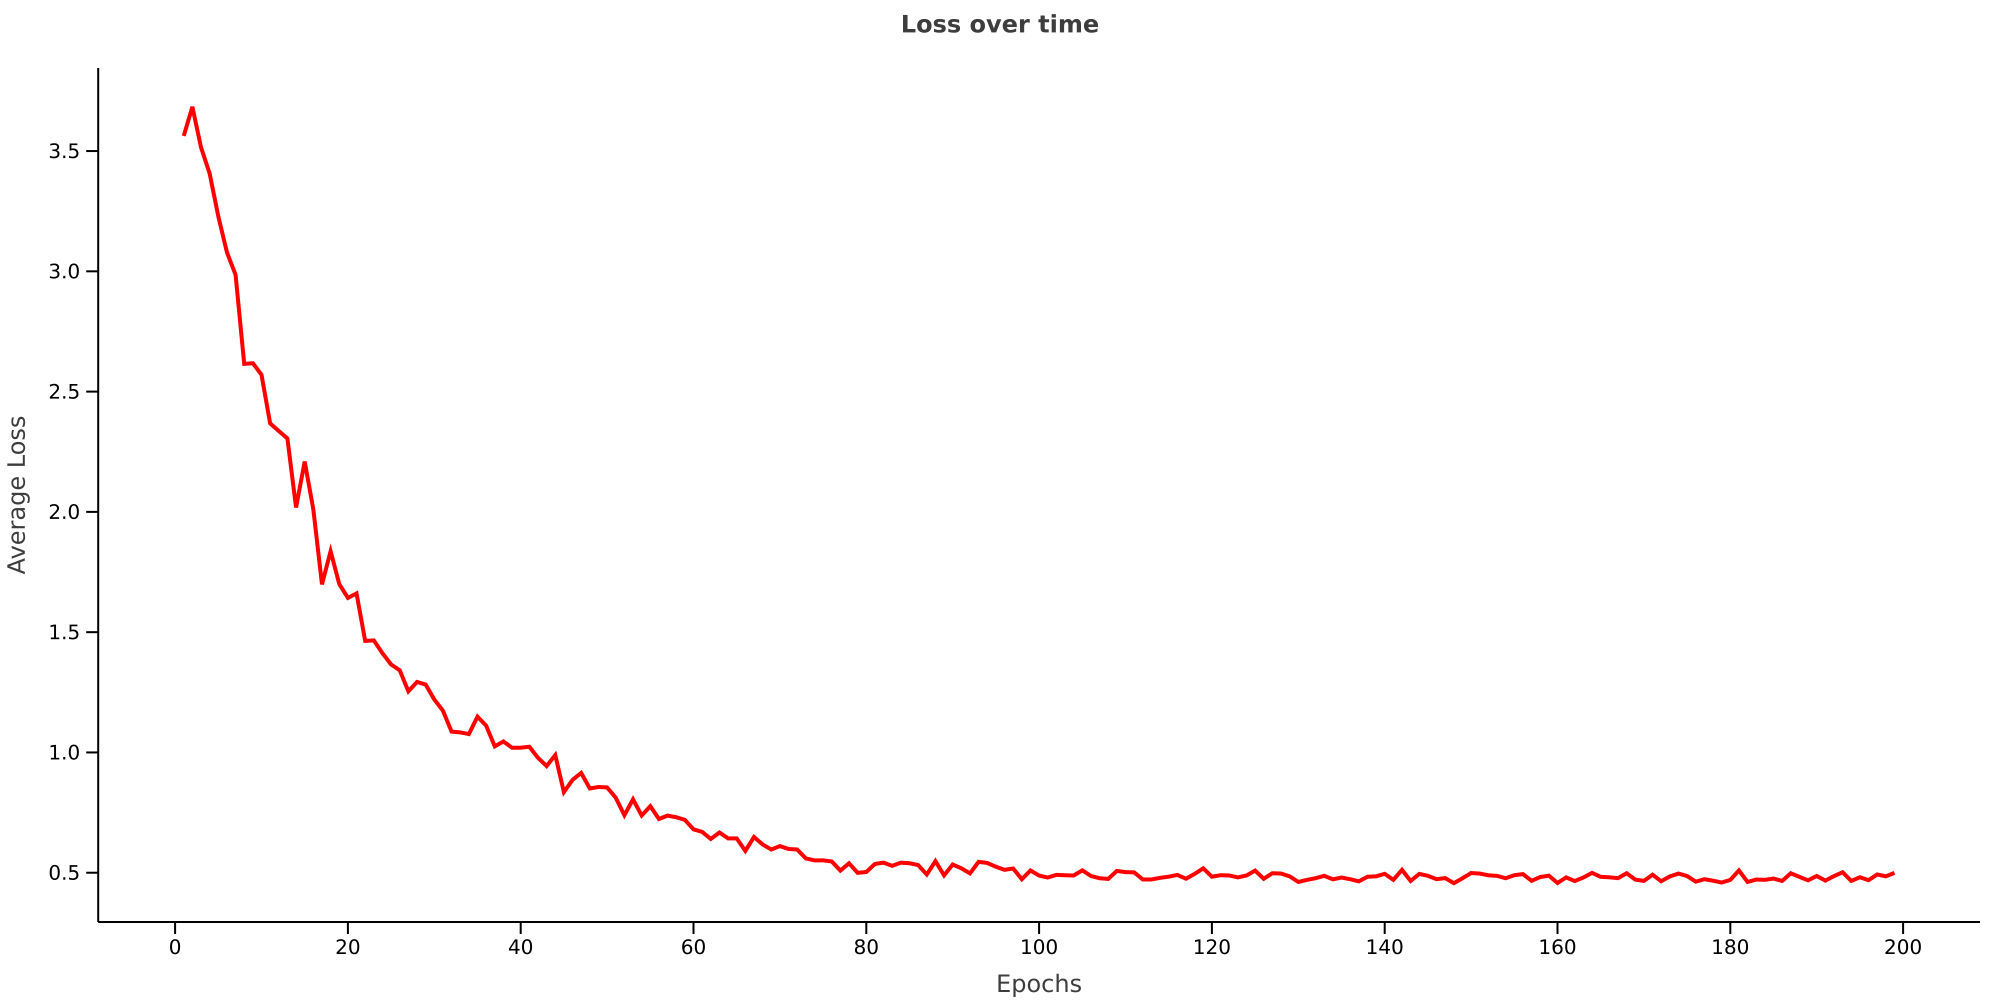
\includegraphics[width=0.70\textwidth]{../figures/training_curve.png}
\caption{Training curve of a single trajectory of gradient descent in parameter space.}
\label{fig:training_curve}
\end{figure}

\begin{table}[H]
\begin{tabular}{ll}
\digraph[scale=0.2]{btree0} {
    graph ["rankdir"="LR","bgcolor"="transparent"];
    "97652294" ["color"="black","fontcolor"="black","fontname"="Helvetica","fontsize"="20","style"="setlinewidth(2)","label"="*"];
    "1027007693" ["color"="black","fontcolor"="black","fontname"="Helvetica","fontsize"="20","style"="setlinewidth(2)","label"="*"];
    "282432134" ["color"="black","fontcolor"="black","fontname"="Helvetica","fontsize"="20","style"="setlinewidth(2)","label"="+"];
    "1282811396" ["color"="black","fontcolor"="black","fontname"="Helvetica","fontsize"="20","style"="setlinewidth(2)","label"="+"];
    "641853239" ["color"="black","fontcolor"="black","fontname"="Helvetica","fontsize"="20","style"="setlinewidth(2)","label"="+"];
    "1920467934" ["color"="black","fontcolor"="black","fontname"="Helvetica","fontsize"="20","style"="setlinewidth(2)","label"="*"];
    "1883840933" ["color"="black","fontcolor"="black","fontname"="Helvetica","fontsize"="20","style"="setlinewidth(2)","label"="*"];
    "233996206" ["color"="black","fontcolor"="black","fontname"="Helvetica","fontsize"="20","style"="setlinewidth(2)","label"="0.307"];
    "x" ["color"="black","fontcolor"="black","fontname"="Helvetica","fontsize"="20","style"="setlinewidth(2)"];
    "614685048" ["color"="black","fontcolor"="black","fontname"="Helvetica","fontsize"="20","style"="setlinewidth(2)","label"="+"];
    "385337537" ["color"="black","fontcolor"="black","fontname"="Helvetica","fontsize"="20","style"="setlinewidth(2)","label"="-"];
    "265119009" ["color"="black","fontcolor"="black","fontname"="Helvetica","fontsize"="20","style"="setlinewidth(2)","label"="*"];
    "832279283" ["color"="black","fontcolor"="black","fontname"="Helvetica","fontsize"="20","style"="setlinewidth(2)","label"="+"];
    "789219251" ["color"="black","fontcolor"="black","fontname"="Helvetica","fontsize"="20","style"="setlinewidth(2)","label"="-"];
    "1375995437" ["color"="black","fontcolor"="black","fontname"="Helvetica","fontsize"="20","style"="setlinewidth(2)","label"="+"];
    "1434041222" ["color"="black","fontcolor"="black","fontname"="Helvetica","fontsize"="20","style"="setlinewidth(2)","label"="+"];
    "838411509" ["color"="black","fontcolor"="black","fontname"="Helvetica","fontsize"="20","style"="setlinewidth(2)","label"="*"];
    "1338841523" ["color"="black","fontcolor"="black","fontname"="Helvetica","fontsize"="20","style"="setlinewidth(2)","label"="-"];
    "802581203" ["color"="black","fontcolor"="black","fontname"="Helvetica","fontsize"="20","style"="setlinewidth(2)","label"="*"];
    "929776179" ["color"="black","fontcolor"="black","fontname"="Helvetica","fontsize"="20","style"="setlinewidth(2)","label"="-"];
    "2050404090" ["color"="black","fontcolor"="black","fontname"="Helvetica","fontsize"="20","style"="setlinewidth(2)","label"="+"];
    "1561408618" ["color"="black","fontcolor"="black","fontname"="Helvetica","fontsize"="20","style"="setlinewidth(2)","label"="+"];
    "668210649" ["color"="black","fontcolor"="black","fontname"="Helvetica","fontsize"="20","style"="setlinewidth(2)","label"="0.355"];
    "1545087375" ["color"="black","fontcolor"="black","fontname"="Helvetica","fontsize"="20","style"="setlinewidth(2)","label"="0.188"];
    "388043093" ["color"="black","fontcolor"="black","fontname"="Helvetica","fontsize"="20","style"="setlinewidth(2)","label"="0.886"];
    "188576144" ["color"="black","fontcolor"="black","fontname"="Helvetica","fontsize"="20","style"="setlinewidth(2)","label"="-1.08"];
    "266437232" ["color"="black","fontcolor"="black","fontname"="Helvetica","fontsize"="20","style"="setlinewidth(2)","label"="0.188"];
    "500772834" ["color"="black","fontcolor"="black","fontname"="Helvetica","fontsize"="20","style"="setlinewidth(2)","label"="1.0"];
    "1691538257" ["color"="black","fontcolor"="black","fontname"="Helvetica","fontsize"="20","style"="setlinewidth(2)","label"="pow"];
    "1335505684" ["color"="black","fontcolor"="black","fontname"="Helvetica","fontsize"="20","style"="setlinewidth(2)","label"="1.555"];
    "1226204845" ["color"="black","fontcolor"="black","fontname"="Helvetica","fontsize"="20","style"="setlinewidth(2)","label"="-"];
    "1" ["color"="black","fontcolor"="black","fontname"="Helvetica","fontsize"="20","style"="setlinewidth(2)","label"="One"];
    "1027007693" -> "97652294" ["color"="blue","arrowhead"="normal","style"="setlinewidth(2)"];
    "282432134" -> "1027007693" ["color"="blue","arrowhead"="normal","style"="setlinewidth(2)"];
    "1282811396" -> "282432134" ["color"="blue","arrowhead"="normal","style"="setlinewidth(2)"];
    "641853239" -> "1282811396" ["color"="blue","arrowhead"="normal","style"="setlinewidth(2)"];
    "1920467934" -> "641853239" ["color"="blue","arrowhead"="normal","style"="setlinewidth(2)"];
    "1883840933" -> "1920467934" ["color"="blue","arrowhead"="normal","style"="setlinewidth(2)"];
    "233996206" -> "1883840933" ["color"="blue","arrowhead"="normal","style"="setlinewidth(2)"];
    "x" -> "1883840933" ["color"="red","arrowhead"="normal","style"="setlinewidth(2)"];
    "x" -> "614685048" ["color"="blue","arrowhead"="normal","style"="setlinewidth(2)"];
    "x" -> "385337537" ["color"="black","arrowhead"="normal","style"="setlinewidth(2)"];
    "x" -> "265119009" ["color"="red","arrowhead"="normal","style"="setlinewidth(2)"];
    "x" -> "1375995437" ["color"="blue","arrowhead"="normal","style"="setlinewidth(2)"];
    "x" -> "1338841523" ["color"="black","arrowhead"="normal","style"="setlinewidth(2)"];
    "x" -> "802581203" ["color"="blue","arrowhead"="normal","style"="setlinewidth(2)"];
    "x" -> "802581203" ["color"="red","arrowhead"="normal","style"="setlinewidth(2)"];
    "x" -> "2050404090" ["color"="blue","arrowhead"="normal","style"="setlinewidth(2)"];
    "614685048" -> "1920467934" ["color"="red","arrowhead"="normal","style"="setlinewidth(2)"];
    "385337537" -> "614685048" ["color"="red","arrowhead"="normal","style"="setlinewidth(2)"];
    "265119009" -> "832279283" ["color"="blue","arrowhead"="normal","style"="setlinewidth(2)"];
    "832279283" -> "789219251" ["color"="black","arrowhead"="normal","style"="setlinewidth(2)"];
    "789219251" -> "641853239" ["color"="red","arrowhead"="normal","style"="setlinewidth(2)"];
    "1375995437" -> "1434041222" ["color"="blue","arrowhead"="normal","style"="setlinewidth(2)"];
    "1434041222" -> "838411509" ["color"="blue","arrowhead"="normal","style"="setlinewidth(2)"];
    "838411509" -> "1282811396" ["color"="red","arrowhead"="normal","style"="setlinewidth(2)"];
    "1338841523" -> "1375995437" ["color"="red","arrowhead"="normal","style"="setlinewidth(2)"];
    "802581203" -> "929776179" ["color"="black","arrowhead"="normal","style"="setlinewidth(2)"];
    "929776179" -> "1434041222" ["color"="red","arrowhead"="normal","style"="setlinewidth(2)"];
    "2050404090" -> "1561408618" ["color"="blue","arrowhead"="normal","style"="setlinewidth(2)"];
    "1561408618" -> "838411509" ["color"="red","arrowhead"="normal","style"="setlinewidth(2)"];
    "668210649" -> "265119009" ["color"="blue","arrowhead"="normal","style"="setlinewidth(2)"];
    "1545087375" -> "832279283" ["color"="red","arrowhead"="normal","style"="setlinewidth(2)"];
    "388043093" -> "2050404090" ["color"="red","arrowhead"="normal","style"="setlinewidth(2)"];
    "188576144" -> "1561408618" ["color"="red","arrowhead"="normal","style"="setlinewidth(2)"];
    "266437232" -> "282432134" ["color"="red","arrowhead"="normal","style"="setlinewidth(2)"];
    "500772834" -> "1027007693" ["color"="red","arrowhead"="normal","style"="setlinewidth(2)"];
    "1691538257" -> "97652294" ["color"="red","arrowhead"="normal","style"="setlinewidth(2)"];
    "1335505684" -> "1691538257" ["color"="blue","arrowhead"="normal","style"="setlinewidth(2)"];
    "1226204845" -> "1691538257" ["color"="red","arrowhead"="normal","style"="setlinewidth(2)"];
    "1" -> "1226204845" ["color"="black","arrowhead"="normal","style"="setlinewidth(2)"];
} & \begin{tikzpicture} \begin{axis}[title={}, width=0.4\textwidth, height=5cm, xlabel=$x$, ylabel=$y$, align=center] \addplot table [mark=none, x index=0, y index=1, col sep=comma] {../data/btree_rand0.csv}; \end{axis} \end{tikzpicture} \\
\digraph[scale=0.2]{btree1} {
    graph ["rankdir"="LR","bgcolor"="transparent"];
    "306115458" ["color"="black","fontcolor"="black","fontname"="Helvetica","fontsize"="20","style"="setlinewidth(2)","label"="*"];
    "944427387" ["color"="black","fontcolor"="black","fontname"="Helvetica","fontsize"="20","style"="setlinewidth(2)","label"="*"];
    "521081105" ["color"="black","fontcolor"="black","fontname"="Helvetica","fontsize"="20","style"="setlinewidth(2)","label"="+"];
    "1907431275" ["color"="black","fontcolor"="black","fontname"="Helvetica","fontsize"="20","style"="setlinewidth(2)","label"="+"];
    "1637061418" ["color"="black","fontcolor"="black","fontname"="Helvetica","fontsize"="20","style"="setlinewidth(2)","label"="+"];
    "1686100174" ["color"="black","fontcolor"="black","fontname"="Helvetica","fontsize"="20","style"="setlinewidth(2)","label"="+"];
    "22671767" ["color"="black","fontcolor"="black","fontname"="Helvetica","fontsize"="20","style"="setlinewidth(2)","label"="+"];
    "2024453272" ["color"="black","fontcolor"="black","fontname"="Helvetica","fontsize"="20","style"="setlinewidth(2)","label"="0.108"];
    "x" ["color"="black","fontcolor"="black","fontname"="Helvetica","fontsize"="20","style"="setlinewidth(2)"];
    "1374026904" ["color"="black","fontcolor"="black","fontname"="Helvetica","fontsize"="20","style"="setlinewidth(2)","label"="*"];
    "536765369" ["color"="black","fontcolor"="black","fontname"="Helvetica","fontsize"="20","style"="setlinewidth(2)","label"="+"];
    "317071334" ["color"="black","fontcolor"="black","fontname"="Helvetica","fontsize"="20","style"="setlinewidth(2)","label"="+"];
    "1224347463" ["color"="black","fontcolor"="black","fontname"="Helvetica","fontsize"="20","style"="setlinewidth(2)","label"="+"];
    "1472465" ["color"="black","fontcolor"="black","fontname"="Helvetica","fontsize"="20","style"="setlinewidth(2)","label"="+"];
    "2129221032" ["color"="black","fontcolor"="black","fontname"="Helvetica","fontsize"="20","style"="setlinewidth(2)","label"="*"];
    "1831477404" ["color"="black","fontcolor"="black","fontname"="Helvetica","fontsize"="20","style"="setlinewidth(2)","label"="+"];
    "1580297332" ["color"="black","fontcolor"="black","fontname"="Helvetica","fontsize"="20","style"="setlinewidth(2)","label"="-"];
    "1966250569" ["color"="black","fontcolor"="black","fontname"="Helvetica","fontsize"="20","style"="setlinewidth(2)","label"="-"];
    "1125381564" ["color"="black","fontcolor"="black","fontname"="Helvetica","fontsize"="20","style"="setlinewidth(2)","label"="+"];
    "370440646" ["color"="black","fontcolor"="black","fontname"="Helvetica","fontsize"="20","style"="setlinewidth(2)","label"="*"];
    "2005733474" ["color"="black","fontcolor"="black","fontname"="Helvetica","fontsize"="20","style"="setlinewidth(2)","label"="-"];
    "511717113" ["color"="black","fontcolor"="black","fontname"="Helvetica","fontsize"="20","style"="setlinewidth(2)","label"="+"];
    "98394724" ["color"="black","fontcolor"="black","fontname"="Helvetica","fontsize"="20","style"="setlinewidth(2)","label"="-0.64"];
    "2085002312" ["color"="black","fontcolor"="black","fontname"="Helvetica","fontsize"="20","style"="setlinewidth(2)","label"="0.186"];
    "1791045777" ["color"="black","fontcolor"="black","fontname"="Helvetica","fontsize"="20","style"="setlinewidth(2)","label"="0.308"];
    "2130772866" ["color"="black","fontcolor"="black","fontname"="Helvetica","fontsize"="20","style"="setlinewidth(2)","label"="0.638"];
    "728739494" ["color"="black","fontcolor"="black","fontname"="Helvetica","fontsize"="20","style"="setlinewidth(2)","label"="0.119"];
    "1237550792" ["color"="black","fontcolor"="black","fontname"="Helvetica","fontsize"="20","style"="setlinewidth(2)","label"="0.518"];
    "1712943792" ["color"="black","fontcolor"="black","fontname"="Helvetica","fontsize"="20","style"="setlinewidth(2)","label"="1.0"];
    "842741472" ["color"="black","fontcolor"="black","fontname"="Helvetica","fontsize"="20","style"="setlinewidth(2)","label"="pow"];
    "1766505436" ["color"="black","fontcolor"="black","fontname"="Helvetica","fontsize"="20","style"="setlinewidth(2)","label"="2.930"];
    "1164440413" ["color"="black","fontcolor"="black","fontname"="Helvetica","fontsize"="20","style"="setlinewidth(2)","label"="-"];
    "1" ["color"="black","fontcolor"="black","fontname"="Helvetica","fontsize"="20","style"="setlinewidth(2)","label"="One"];
    "944427387" -> "306115458" ["color"="blue","arrowhead"="normal","style"="setlinewidth(2)"];
    "521081105" -> "944427387" ["color"="blue","arrowhead"="normal","style"="setlinewidth(2)"];
    "1907431275" -> "521081105" ["color"="blue","arrowhead"="normal","style"="setlinewidth(2)"];
    "1637061418" -> "1907431275" ["color"="blue","arrowhead"="normal","style"="setlinewidth(2)"];
    "1686100174" -> "1637061418" ["color"="blue","arrowhead"="normal","style"="setlinewidth(2)"];
    "22671767" -> "1686100174" ["color"="blue","arrowhead"="normal","style"="setlinewidth(2)"];
    "2024453272" -> "22671767" ["color"="blue","arrowhead"="normal","style"="setlinewidth(2)"];
    "x" -> "22671767" ["color"="red","arrowhead"="normal","style"="setlinewidth(2)"];
    "x" -> "1374026904" ["color"="red","arrowhead"="normal","style"="setlinewidth(2)"];
    "x" -> "317071334" ["color"="blue","arrowhead"="normal","style"="setlinewidth(2)"];
    "x" -> "317071334" ["color"="red","arrowhead"="normal","style"="setlinewidth(2)"];
    "x" -> "1224347463" ["color"="red","arrowhead"="normal","style"="setlinewidth(2)"];
    "x" -> "1831477404" ["color"="blue","arrowhead"="normal","style"="setlinewidth(2)"];
    "x" -> "1966250569" ["color"="black","arrowhead"="normal","style"="setlinewidth(2)"];
    "x" -> "1125381564" ["color"="blue","arrowhead"="normal","style"="setlinewidth(2)"];
    "x" -> "2005733474" ["color"="black","arrowhead"="normal","style"="setlinewidth(2)"];
    "1374026904" -> "536765369" ["color"="blue","arrowhead"="normal","style"="setlinewidth(2)"];
    "536765369" -> "1637061418" ["color"="red","arrowhead"="normal","style"="setlinewidth(2)"];
    "317071334" -> "536765369" ["color"="red","arrowhead"="normal","style"="setlinewidth(2)"];
    "1224347463" -> "1472465" ["color"="blue","arrowhead"="normal","style"="setlinewidth(2)"];
    "1472465" -> "2129221032" ["color"="blue","arrowhead"="normal","style"="setlinewidth(2)"];
    "2129221032" -> "1907431275" ["color"="red","arrowhead"="normal","style"="setlinewidth(2)"];
    "1831477404" -> "1580297332" ["color"="black","arrowhead"="normal","style"="setlinewidth(2)"];
    "1580297332" -> "1472465" ["color"="red","arrowhead"="normal","style"="setlinewidth(2)"];
    "1966250569" -> "1831477404" ["color"="red","arrowhead"="normal","style"="setlinewidth(2)"];
    "1125381564" -> "370440646" ["color"="blue","arrowhead"="normal","style"="setlinewidth(2)"];
    "370440646" -> "2129221032" ["color"="red","arrowhead"="normal","style"="setlinewidth(2)"];
    "2005733474" -> "511717113" ["color"="red","arrowhead"="normal","style"="setlinewidth(2)"];
    "511717113" -> "370440646" ["color"="red","arrowhead"="normal","style"="setlinewidth(2)"];
    "98394724" -> "1686100174" ["color"="red","arrowhead"="normal","style"="setlinewidth(2)"];
    "2085002312" -> "1374026904" ["color"="blue","arrowhead"="normal","style"="setlinewidth(2)"];
    "1791045777" -> "1224347463" ["color"="blue","arrowhead"="normal","style"="setlinewidth(2)"];
    "2130772866" -> "1125381564" ["color"="red","arrowhead"="normal","style"="setlinewidth(2)"];
    "728739494" -> "511717113" ["color"="blue","arrowhead"="normal","style"="setlinewidth(2)"];
    "1237550792" -> "521081105" ["color"="red","arrowhead"="normal","style"="setlinewidth(2)"];
    "1712943792" -> "944427387" ["color"="red","arrowhead"="normal","style"="setlinewidth(2)"];
    "842741472" -> "306115458" ["color"="red","arrowhead"="normal","style"="setlinewidth(2)"];
    "1766505436" -> "842741472" ["color"="blue","arrowhead"="normal","style"="setlinewidth(2)"];
    "1164440413" -> "842741472" ["color"="red","arrowhead"="normal","style"="setlinewidth(2)"];
    "1" -> "1164440413" ["color"="black","arrowhead"="normal","style"="setlinewidth(2)"];
} & \begin{tikzpicture} \begin{axis}[title={}, width=0.4\textwidth, height=5cm, xlabel=$x$, ylabel=$y$, align=center] \addplot table [mark=none, x index=0, y index=1, col sep=comma] {../data/btree_rand1.csv}; \end{axis} \end{tikzpicture} \\
\digraph[scale=0.2]{btree2} {
    graph ["rankdir"="LR","bgcolor"="transparent"];
    "1007412025" ["color"="black","fontcolor"="black","fontname"="Helvetica","fontsize"="20","style"="setlinewidth(2)","label"="*"];
    "2053591126" ["color"="black","fontcolor"="black","fontname"="Helvetica","fontsize"="20","style"="setlinewidth(2)","label"="*"];
    "231756373" ["color"="black","fontcolor"="black","fontname"="Helvetica","fontsize"="20","style"="setlinewidth(2)","label"="+"];
    "887750041" ["color"="black","fontcolor"="black","fontname"="Helvetica","fontsize"="20","style"="setlinewidth(2)","label"="+"];
    "1010953501" ["color"="black","fontcolor"="black","fontname"="Helvetica","fontsize"="20","style"="setlinewidth(2)","label"="+"];
    "1423561005" ["color"="black","fontcolor"="black","fontname"="Helvetica","fontsize"="20","style"="setlinewidth(2)","label"="+"];
    "943870983" ["color"="black","fontcolor"="black","fontname"="Helvetica","fontsize"="20","style"="setlinewidth(2)","label"="+"];
    "x" ["color"="black","fontcolor"="black","fontname"="Helvetica","fontsize"="20","style"="setlinewidth(2)"];
    "1084502906" ["color"="black","fontcolor"="black","fontname"="Helvetica","fontsize"="20","style"="setlinewidth(2)","label"="-"];
    "1881561036" ["color"="black","fontcolor"="black","fontname"="Helvetica","fontsize"="20","style"="setlinewidth(2)","label"="+"];
    "52908367" ["color"="black","fontcolor"="black","fontname"="Helvetica","fontsize"="20","style"="setlinewidth(2)","label"="*"];
    "1279271200" ["color"="black","fontcolor"="black","fontname"="Helvetica","fontsize"="20","style"="setlinewidth(2)","label"="-"];
    "587153993" ["color"="black","fontcolor"="black","fontname"="Helvetica","fontsize"="20","style"="setlinewidth(2)","label"="+"];
    "1613095350" ["color"="black","fontcolor"="black","fontname"="Helvetica","fontsize"="20","style"="setlinewidth(2)","label"="-"];
    "1971764991" ["color"="black","fontcolor"="black","fontname"="Helvetica","fontsize"="20","style"="setlinewidth(2)","label"="+"];
    "1276261147" ["color"="black","fontcolor"="black","fontname"="Helvetica","fontsize"="20","style"="setlinewidth(2)","label"="+"];
    "18242360" ["color"="black","fontcolor"="black","fontname"="Helvetica","fontsize"="20","style"="setlinewidth(2)","label"="*"];
    "1527953000" ["color"="black","fontcolor"="black","fontname"="Helvetica","fontsize"="20","style"="setlinewidth(2)","label"="-"];
    "135640095" ["color"="black","fontcolor"="black","fontname"="Helvetica","fontsize"="20","style"="setlinewidth(2)","label"="*"];
    "1632682988" ["color"="black","fontcolor"="black","fontname"="Helvetica","fontsize"="20","style"="setlinewidth(2)","label"="*"];
    "359922172" ["color"="black","fontcolor"="black","fontname"="Helvetica","fontsize"="20","style"="setlinewidth(2)","label"="+"];
    "1136419747" ["color"="black","fontcolor"="black","fontname"="Helvetica","fontsize"="20","style"="setlinewidth(2)","label"="0.375"];
    "1785507932" ["color"="black","fontcolor"="black","fontname"="Helvetica","fontsize"="20","style"="setlinewidth(2)","label"="0.791"];
    "757004314" ["color"="black","fontcolor"="black","fontname"="Helvetica","fontsize"="20","style"="setlinewidth(2)","label"="1.261"];
    "996796369" ["color"="black","fontcolor"="black","fontname"="Helvetica","fontsize"="20","style"="setlinewidth(2)","label"="-0.65"];
    "1430439149" ["color"="black","fontcolor"="black","fontname"="Helvetica","fontsize"="20","style"="setlinewidth(2)","label"="0.236"];
    "1153447573" ["color"="black","fontcolor"="black","fontname"="Helvetica","fontsize"="20","style"="setlinewidth(2)","label"="0.494"];
    "1786294176" ["color"="black","fontcolor"="black","fontname"="Helvetica","fontsize"="20","style"="setlinewidth(2)","label"="-0.23"];
    "2082351774" ["color"="black","fontcolor"="black","fontname"="Helvetica","fontsize"="20","style"="setlinewidth(2)","label"="1.0"];
    "1730704097" ["color"="black","fontcolor"="black","fontname"="Helvetica","fontsize"="20","style"="setlinewidth(2)","label"="pow"];
    "1062635358" ["color"="black","fontcolor"="black","fontname"="Helvetica","fontsize"="20","style"="setlinewidth(2)","label"="3.506"];
    "265321659" ["color"="black","fontcolor"="black","fontname"="Helvetica","fontsize"="20","style"="setlinewidth(2)","label"="-"];
    "1" ["color"="black","fontcolor"="black","fontname"="Helvetica","fontsize"="20","style"="setlinewidth(2)","label"="One"];
    "2053591126" -> "1007412025" ["color"="blue","arrowhead"="normal","style"="setlinewidth(2)"];
    "231756373" -> "2053591126" ["color"="blue","arrowhead"="normal","style"="setlinewidth(2)"];
    "887750041" -> "231756373" ["color"="blue","arrowhead"="normal","style"="setlinewidth(2)"];
    "1010953501" -> "887750041" ["color"="blue","arrowhead"="normal","style"="setlinewidth(2)"];
    "1423561005" -> "1010953501" ["color"="blue","arrowhead"="normal","style"="setlinewidth(2)"];
    "943870983" -> "1423561005" ["color"="blue","arrowhead"="normal","style"="setlinewidth(2)"];
    "x" -> "943870983" ["color"="blue","arrowhead"="normal","style"="setlinewidth(2)"];
    "x" -> "1084502906" ["color"="black","arrowhead"="normal","style"="setlinewidth(2)"];
    "x" -> "52908367" ["color"="blue","arrowhead"="normal","style"="setlinewidth(2)"];
    "x" -> "52908367" ["color"="red","arrowhead"="normal","style"="setlinewidth(2)"];
    "x" -> "1971764991" ["color"="blue","arrowhead"="normal","style"="setlinewidth(2)"];
    "x" -> "135640095" ["color"="blue","arrowhead"="normal","style"="setlinewidth(2)"];
    "x" -> "1632682988" ["color"="blue","arrowhead"="normal","style"="setlinewidth(2)"];
    "x" -> "1632682988" ["color"="red","arrowhead"="normal","style"="setlinewidth(2)"];
    "1084502906" -> "1881561036" ["color"="red","arrowhead"="normal","style"="setlinewidth(2)"];
    "1881561036" -> "1423561005" ["color"="red","arrowhead"="normal","style"="setlinewidth(2)"];
    "52908367" -> "1279271200" ["color"="black","arrowhead"="normal","style"="setlinewidth(2)"];
    "1279271200" -> "587153993" ["color"="red","arrowhead"="normal","style"="setlinewidth(2)"];
    "587153993" -> "1613095350" ["color"="black","arrowhead"="normal","style"="setlinewidth(2)"];
    "1613095350" -> "1010953501" ["color"="red","arrowhead"="normal","style"="setlinewidth(2)"];
    "1971764991" -> "1276261147" ["color"="blue","arrowhead"="normal","style"="setlinewidth(2)"];
    "1276261147" -> "18242360" ["color"="blue","arrowhead"="normal","style"="setlinewidth(2)"];
    "18242360" -> "1527953000" ["color"="black","arrowhead"="normal","style"="setlinewidth(2)"];
    "1527953000" -> "887750041" ["color"="red","arrowhead"="normal","style"="setlinewidth(2)"];
    "135640095" -> "1276261147" ["color"="red","arrowhead"="normal","style"="setlinewidth(2)"];
    "1632682988" -> "359922172" ["color"="blue","arrowhead"="normal","style"="setlinewidth(2)"];
    "359922172" -> "18242360" ["color"="red","arrowhead"="normal","style"="setlinewidth(2)"];
    "1136419747" -> "943870983" ["color"="red","arrowhead"="normal","style"="setlinewidth(2)"];
    "1785507932" -> "1881561036" ["color"="blue","arrowhead"="normal","style"="setlinewidth(2)"];
    "757004314" -> "587153993" ["color"="blue","arrowhead"="normal","style"="setlinewidth(2)"];
    "996796369" -> "1971764991" ["color"="red","arrowhead"="normal","style"="setlinewidth(2)"];
    "1430439149" -> "135640095" ["color"="red","arrowhead"="normal","style"="setlinewidth(2)"];
    "1153447573" -> "359922172" ["color"="red","arrowhead"="normal","style"="setlinewidth(2)"];
    "1786294176" -> "231756373" ["color"="red","arrowhead"="normal","style"="setlinewidth(2)"];
    "2082351774" -> "2053591126" ["color"="red","arrowhead"="normal","style"="setlinewidth(2)"];
    "1730704097" -> "1007412025" ["color"="red","arrowhead"="normal","style"="setlinewidth(2)"];
    "1062635358" -> "1730704097" ["color"="blue","arrowhead"="normal","style"="setlinewidth(2)"];
    "265321659" -> "1730704097" ["color"="red","arrowhead"="normal","style"="setlinewidth(2)"];
    "1" -> "265321659" ["color"="black","arrowhead"="normal","style"="setlinewidth(2)"];
} & \begin{tikzpicture} \begin{axis}[title={}, width=0.4\textwidth, height=5cm, xlabel=$x$, ylabel=$y$, align=center] \addplot table [mark=none, x index=0, y index=1, col sep=comma] {../data/btree_rand2.csv}; \end{axis} \end{tikzpicture}
\end{tabular}
\caption{\label{tab:btrees} Some DFGs generated by \autoref{eq:btree_gen} with accompanying 2D plots.}
\end{table}

\begin{figure}
\begin{tikzpicture} \begin{axis}[title={Average Errors per 1k Evaluations for Random Sampling Strategy}, width=0.8\textwidth, height=5cm, xlabel=$\text{Error threshold}$, ylabel=$\text{Errors/eval}$, align=center] \addplot table [mark=none, x index=0, y index=1, col sep=comma] {../data/urand_eff0.csv}; \end{axis} \end{tikzpicture} \\
\end{figure}


violations for exceeding threshold
compare baseline w.r.t. finding
leave out intervals, search to find regions. compare # of samples

\section{Conclusion}

In this chapter we have visited some interesting ideas for validating intelligent systems from the perspective of software engineering and machine learning. We have seen a curious resemblance between some new and old ideas in adversarial learning and fuzz testing. We have proposed a framework for evaluating differentiable programs in a low-cost, data-driven manner and suggest some intriguing directions for future research.

\begin{figure}
\centering
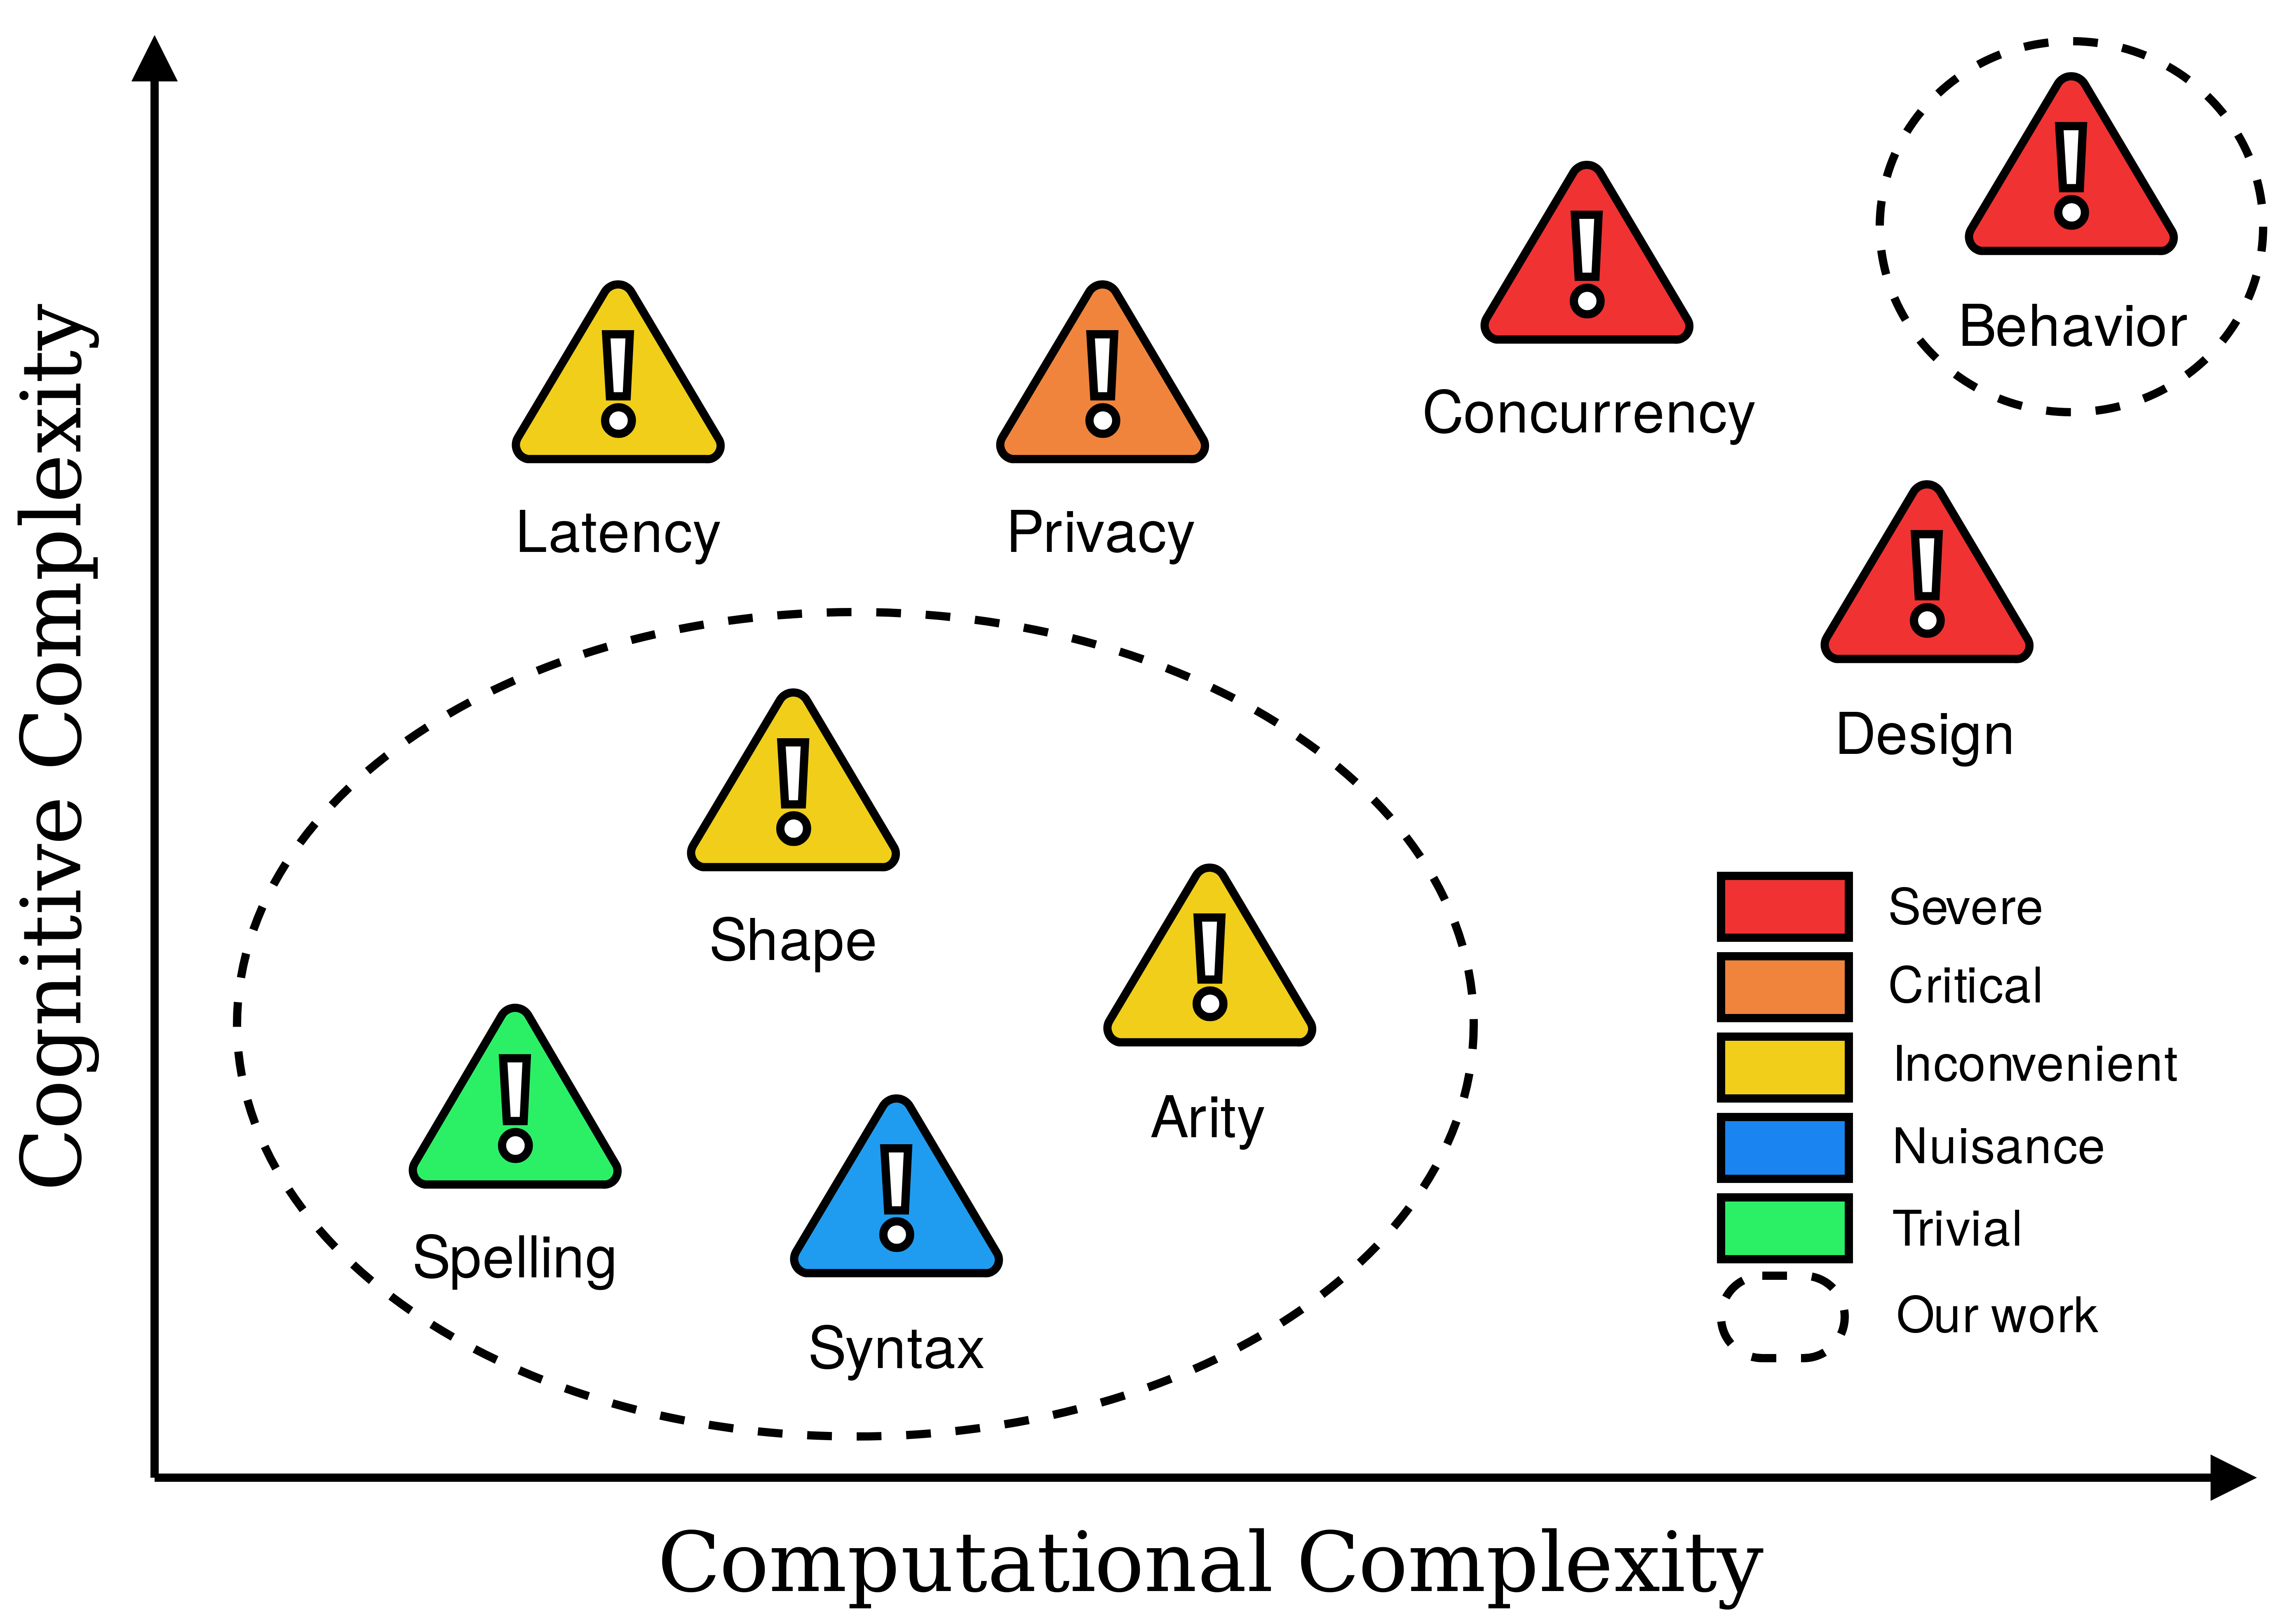
\includegraphics[width=0.60\textwidth]{../figures/verification_complexity.png}
\caption{Complexity of detecting various types of programming errors.}
\label{fig:verification_complexity}
\end{figure}

Type systems, compilers and fuzzers are all part of a broader class of validation and verification tools. The goal of these tools is to provide feedback as early as possible. Some errors (e.g. syntactical errors), are minor nuisances and can be quickly detected with a good incremental parser (\autoref{subsec:the-parser}). Others, as shown in~\autoref{fig:verification_complexity}, are more complex but can be detected by spending computation. We argue this computational cost is often justified as undetected bugs can have catastrophic consequences. Spending computation frees up valuable cognitive resources better spent on more challenging tasks downstream. Studies have shown bugs detected early in development are more likely to be fixed~\citep{distefano2019scaling} -- saving minutes in development could save lives during operation.

Learning capabilities will play a crucial role in autonomous systems. As today's engineers begin to incorporate learning in tomorrow's safety-critical robotic systems, we believe the increased assurance provided by intelligent validation and verification tools will be indispensable for the widespread deployment of these complex adaptive cyberphysical systems.
